\subsection*{Teil C: Koordinatensystem (20 Minuten)}

\begin{enumerate}[resume, label=\arabic*.]
    \item \textbf{Zeichne ein Koordinatensystem und trage folgende Punkte ein:}

    $A(2|3), B(-1|2), C(3|-2), D(-2|-1), E(0|2), F(3|0)$

    \begin{center}
        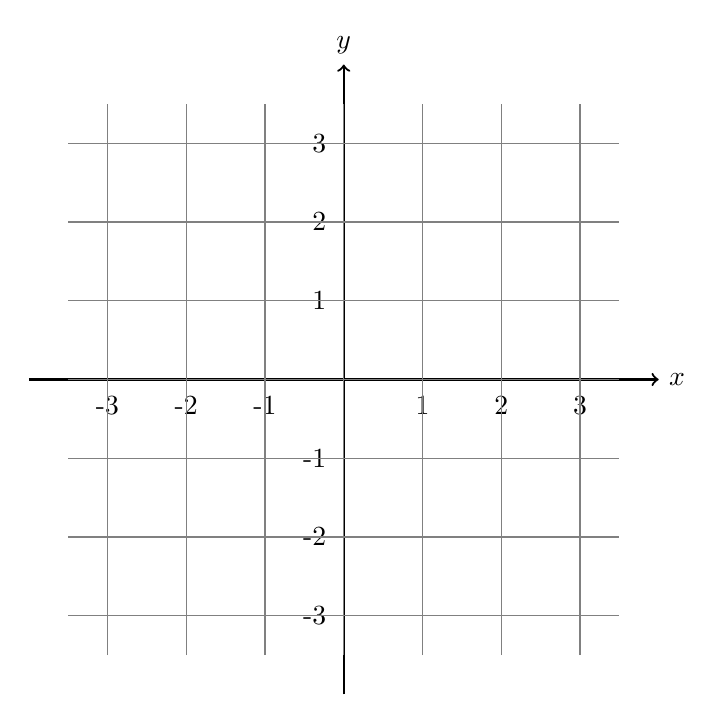
\begin{tikzpicture}[scale=1]
            \draw[thick,->] (-4,0) -- (4,0) node[right] {$x$};
            \draw[thick,->] (0,-4) -- (0,4) node[above] {$y$};
            \foreach \x in {-3,-2,-1,1,2,3}
            \draw (\x,0.1) -- (\x,-0.1) node[below] {\x};
            \foreach \y in {-3,-2,-1,1,2,3}
            \draw (0.1,\y) -- (-0.1,\y) node[left] {\y};
            \draw[thin,gray,step=1] (-3.5,-3.5) grid (3.5,3.5);
        \end{tikzpicture}
    \end{center}

    \vspace{0.5cm}

    \item \textbf{Lies die Koordinaten der eingezeichneten Punkte ab:}

    \begin{center}
        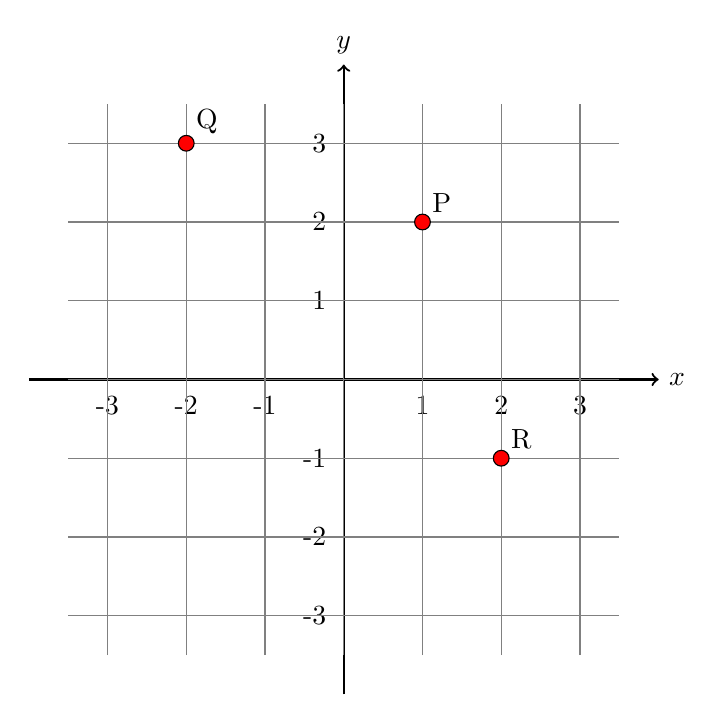
\begin{tikzpicture}[scale=1]
            \draw[thick,->] (-4,0) -- (4,0) node[right] {$x$};
            \draw[thick,->] (0,-4) -- (0,4) node[above] {$y$};
            \foreach \x in {-3,-2,-1,1,2,3}
            \draw (\x,0.1) -- (\x,-0.1) node[below] {\x};
            \foreach \y in {-3,-2,-1,1,2,3}
            \draw (0.1,\y) -- (-0.1,\y) node[left] {\y};
            \draw[thin,gray,step=1] (-3.5,-3.5) grid (3.5,3.5);
            % Punkte zum Ablesen
            \draw[fill=red] (1,2) circle (0.1) node[above right] {P};
            \draw[fill=red] (-2,3) circle (0.1) node[above right] {Q};
            \draw[fill=red] (2,-1) circle (0.1) node[above right] {R};
        \end{tikzpicture}
    \end{center}

    \begin{itemize}
        \item Punkt P: (\underline{\hspace{1.5cm}}\|\underline{\hspace{1.5cm}})
        \item Punkt Q: (\underline{\hspace{1.5cm}}\|\underline{\hspace{1.5cm}})
        \item Punkt R: (\underline{\hspace{1.5cm}}\|\underline{\hspace{1.5cm}})
    \end{itemize}
\end{enumerate}